\documentclass[border=10pt]{standalone}
\usepackage[T1]{fontenc}
\usepackage{amsmath,amsfonts}
\usepackage{tikz}
\usetikzlibrary{shapes.geometric} % Cylinder
\usetikzlibrary{shadows.blur,arrows.meta,bending,positioning}
\usetikzlibrary{%
	calc,%
	decorations.pathmorphing,%
	fadings,%
	shadings,
   decorations.pathreplacing,calligraphy
}
\usepackage{xcolor}
\makeatletter% from https://tex.stackexchange.com/a/39698/121799
\def\grd@save@target#1{%
  \def\grd@target{#1}}
\def\grd@save@start#1{%
  \def\grd@start{#1}}
\tikzset{
  labeled grid/.style={
    to path={%
      \pgfextra{%
        \edef\grd@@target{(\tikztotarget)}%
        \tikz@scan@one@point\grd@save@target\grd@@target\relax
        \edef\grd@@start{(\tikztostart)}%
        \tikz@scan@one@point\grd@save@start\grd@@start\relax
        \draw[minor help lines] (\tikztostart) grid (\tikztotarget);
        \draw[major help lines] (\tikztostart) grid (\tikztotarget);
        \grd@start
        \pgfmathsetmacro{\grd@xa}{\the\pgf@x/1cm}
        \pgfmathsetmacro{\grd@ya}{\the\pgf@y/1cm}
        \grd@target
        \pgfmathsetmacro{\grd@xb}{\the\pgf@x/1cm}
        \pgfmathsetmacro{\grd@yb}{\the\pgf@y/1cm}
        \pgfmathsetmacro{\grd@xc}{\grd@xa + \pgfkeysvalueof{/tikz/grid with coordinates/major step}}
        \pgfmathsetmacro{\grd@yc}{\grd@ya + \pgfkeysvalueof{/tikz/grid with coordinates/major step}}
        \foreach \x in {\grd@xa,\grd@xc,...,\grd@xb}
        \node[anchor=north] at (\x,\grd@ya) {\pgfmathprintnumber{\x}};
        \foreach \y in {\grd@ya,\grd@yc,...,\grd@yb}
        \node[anchor=east] at (\grd@xa,\y) {\pgfmathprintnumber{\y}};
        \path foreach \x in {\grd@xa,\grd@xc,...,\grd@xb}
        {foreach \y in {\grd@ya,\grd@yc,...,\grd@yb}
         { (\x,\y) node[grid with coordinates/grid label,opacity=0.3] {$(\pgfmathprintnumber{\x},\pgfmathprintnumber{\y})$}}};
      }
    }
  },
  minor help lines/.style={
    help lines,
    step=\pgfkeysvalueof{/tikz/grid with coordinates/minor step},
    draw=none
  },
  major help lines/.style={
    help lines,
    line width=\pgfkeysvalueof{/tikz/grid with coordinates/major line width},
    step=\pgfkeysvalueof{/tikz/grid with coordinates/major step}
  },
  grid with coordinates/.cd,
  minor step/.initial=.2,
  major step/.initial=1,
  major line width/.initial=2pt,
  grid label/.style={below left,scale=0.5,opacity=0.5}
}
\makeatother



\begin{document}
  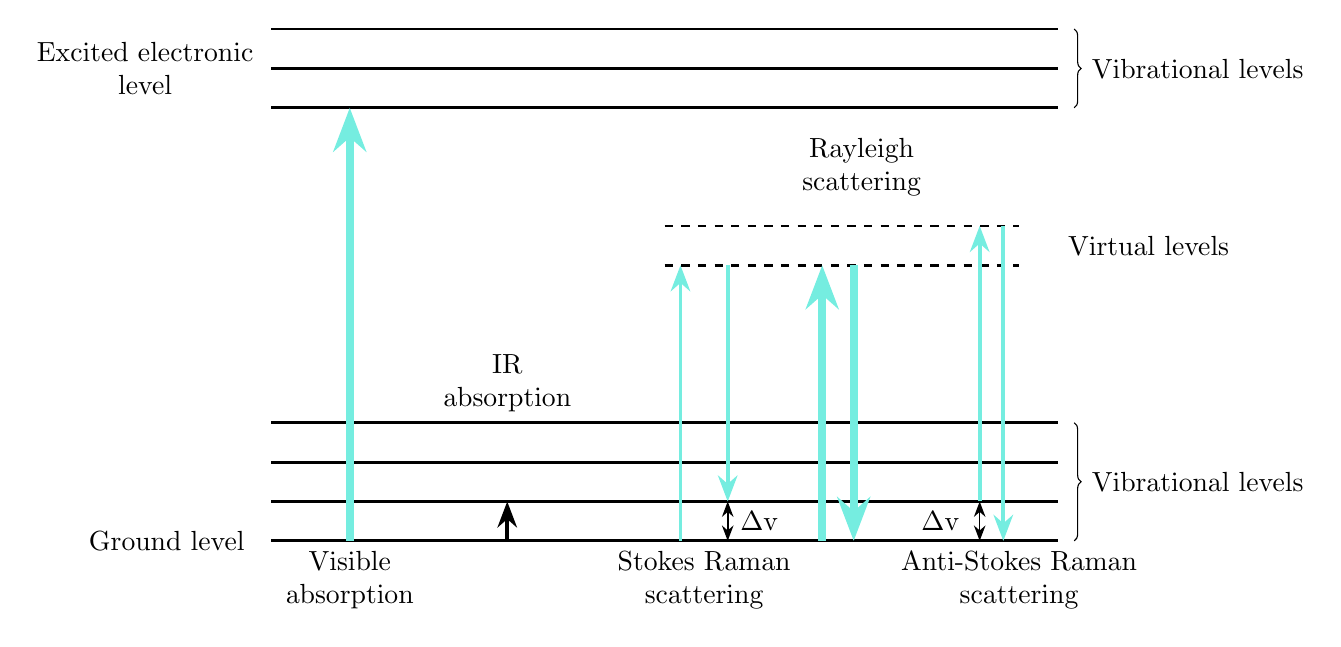
\begin{tikzpicture}

% \begin{scope}[opacity=0.03]
%     \draw(0,0) to[labeled grid] (10,7);    
% \end{scope}
        
    \foreach \x in {5.5,6,6.5}{
      \draw[line width=1pt](0,\x)--(10,\x);
    }

    \draw [decorate,decoration = {brace,mirror}] (10.2,5.5) --  (10.2,6.5);
    \node[anchor=west] at (10.3,6) {Vibrational levels};

    \node[anchor=east, align=center] at (-0.1,6) {Excited electronic\\level};

    \draw[dashed,line width=1pt](5,4)--(9.5,4);
    \draw[dashed,line width=1pt](5,3.5)--(9.5,3.5);
    \node[anchor=west] at (10,3.75) {Virtual levels};

    \foreach \x in {0,0.5,...,1.5}{
        \draw[line width=1pt](0,\x)--(10,\x);
      }

      \definecolor{pcolor}{HTML}{75EDE0}

      \draw[-{Stealth},line width=1mm,pcolor] (1,0)--(1,5.5);
      \draw[-{Stealth},line width=.5mm,pcolor] (5.2,0)--(5.2,3.5);
      \draw[-{Stealth},line width=.5mm,pcolor] (5.8,3.5)--(5.8,0.5);
      \draw[{Stealth}-{Stealth},line width=.2mm,black] (5.8,0)--(5.8,0.5);
      \node at (6.2,0.25) {$\Delta$v};

      \draw[-{Stealth},line width=1mm,pcolor] (7,0)--(7,3.5);
      \draw[-{Stealth},line width=1mm,pcolor] (7.4,3.5)--(7.4,0);

      \draw [decorate,decoration = {brace,mirror}] (10.2,0) --  (10.2,1.5);
      \node[anchor=west] at (10.3,0.75) {Vibrational levels};
      \node[anchor=center,text width=2cm,align=center] at (7.5,4.75) {Rayleigh\\scattering};

      \draw[-{Stealth},line width=.5mm,pcolor] (9,0.5)--(9,4);
      \draw[{Stealth}-{Stealth},line width=.2mm,black] (9,0)--(9,0.5);
      \draw[-{Stealth},line width=.5mm,pcolor] (9.3,4)--(9.3,0);
      \node at (8.5,0.25) {$\Delta$v};

      \node[anchor=center,text width=2cm,align=center] at (3,2) {IR\\absorption};
      \draw[-{Stealth},line width=.5mm] (3,0)--(3,0.5);

      \node[anchor=east,text width=2cm,align=center] at (-0.2,0) {Ground level};

      \node[anchor=center,text width=2cm,align=center] at (1,-0.5) {Visible\\absorption};

      \node[anchor=center,text width=3cm,align=center] at (5.5,-0.5) {Stokes Raman\\scattering};

      \node[anchor=center,text width=3cm,align=center] at (9.5,-0.5) {Anti-Stokes Raman\\scattering};

  \end{tikzpicture}
\end{document}